\section{Efektywne zbieranie logów}
\label{chapter:logs:collecting}

    Nawet małej wielkości system informatyczny jest w stanie wygenerować kilka tysięcy logów w ciągu
    zaledwie kilku godzin swojego działania. Logi systemowe, audyty bezpieczeństwa, logi aplikacji oraz
    logi pochodzące z urządzeń fizycznych - każdy z nich może zawierać informacje potrzebne
    administratorom systemu. 
    
    \subsection{Źródła logów}
    \label{chapter:logs:collecting:source}
    Źródła, z których pochodzą logi można podzielić na dwie główne kategorie:
    \begin{itemize}
        \item[\textbf{push-based}]
            - aplikacja lub urządzenie zapisuje kolejne rekordy do pliku zlokalizowanego
            na tej samej maszynie. Konieczne jest więc zalogowanie się do niej, aby 
            mieć wgląd do tego, co działo się z danym programem. Z tego powodu istnieje
            alternatywna droga, która może być wymienna z pierwszą lub być komplementarna do niej.
            Program może jednocześnie zapisać dane do pliku oraz wysyłać je przez sieć. W tym
            wypadku, konieczne jest posiadanie serwera skonfigurowanego do odbierania logów 
            \cite{logging_log_management}.
        \item[\textbf{pull-based}]
            - podejście odwrotne do omówionego w powyżej. W tym wypadku,
            klientem jest aplikacja, która pobiera logi z monitorowanego programu. Jest ona najczęściej
            implementowana w architekturze \textbf{klient-serwer}\footnote{Klient-Serwer - Model architektury
                systemów. Serwer udostępnia usługi, które wykorzystuje klient, aby zrealizować zadania
                pochodzące od użytkownika systemu}. Inną cechą szczególną jest własnościowy format logu.
            Logi są pobierane z programu aktywnie, w podobny sposób w jaki, na żądanie, realizowana
            jest pewna usługa klienta \cite{logging_log_management}.
    \end{itemize}
    
        \subsubsection{Syslog}
        \label{chapter:logs:collecting:source:syslog}
        Obecnie wiodące rozwiązanie na platformie Unix, umożliwiające efektywne zbieranie logów. 
        W podstawowej wersji składa się on z demona \textbf{syslogd} - usługi
        uruchamianej wraz ze startem systemu operacyjnego i zatrzymywanej przy jego wyłączaniu. 
        Aplikacja, która chce zapisywać logi z jego wykorzystaniem, wykorzystuje bibliotekę \textbf{syslog}.
        Udostępnione przez nią funkcję pozwalają na wygenerowanie odpowiedniego zdarzania, które jest
        w dalszej kolejności wysyłane poprzez socket do działającej usługi \textbf{syslogd}. Możliwe jest
        również wykorzystanie protokołu \textit{UDP} do tego samego celu.
        Nowsze implementacje \textbf{syslog}, takie jak \textbf{rsylog} czy też \textbf{syslog-ng}, 
        wykorzystują protokół \textit{TCP}. Podstawą różnicą między nimi jest bezpieczeństwo. TCP, w stosunku do UDP \cite{logging_log_management}
        gwarantuje w znacznie większym stopniu dostarczenie wiadomości.
        Jego głównymi zaletami jest centralna konfiguracja oraz popularność.
        
        \subsubsection{Windows Event Log}
        \label{chapter:logs:collecting:source:windows_event_log}
        Własnościowe rozwiązanie firmy \textbf{Microsoft}. Dla systemów rodziny \textbf{Windows}
        ma on podobne znaczenie do \textbf{syslog}(\ref{chapter:logs:collecting:source:syslog}),
        dostępnego w systemach Unix'owych. Zastosowaniem tego systemu jest:
        \begin{itemize}
            \item zbieranie logów systemowych,
            \item zbieranie logów aplikacji.
        \end{itemize}
        Jako logi systemowe rozumie się wszelkie wydarzenia pochodzące od samego systemu. W ich skład
        wliczane są między innymi: wydarzenia związane z bezpieczeństwem, np. 
        logowanie użytkownika oraz zdarzenia systemowe, pochodzące z jądra systemu. Aplikacje
        również mogą korzystać \textbf{Windows Event Log}.
        
        \subsubsection{Problem wielu źródeł}
        \label{chapter:logs:collecting:multiple_sources}
        Logi to praktycznie nigdy, wyłączając małe aplikacje, które działają na pojedynczej maszynie,
        jedno źródło danych. W przypadku aplikacji biznesowych mogą być one rozsiane na kilku lub nawet
        kilkunastu różnych serwerach oraz pochodzić z więcej niż jednego programu na nim uruchomionego.
        Przekłada się to, w stosunku 1:1, na kilka lub kilkanaście oddzielnych miejsc źródłowych, z których
        log może zostać pobrany. Jeśli doliczyć do tego logi systemowe (lub inne możliwe rodzaje(\ref{chapter:logs:classification}),
        ilość ta może jeszcze wzrosnąć \cite{guide_to_computer_security_log_management}.

    \subsection{Archiwizowanie logów}
    \label{chapter:logs:collecting:archive}
    Dowolny program generuje logi nieprzerwanie. Zazwyczaj główny miejscem docelowym, gdzie możliwe jest
    przeanalizowanie logów, jest plik tekstowy zapisanych na maszynie gdzie aplikacja funkcjonuje.
    Niestety nie jest to równoznaczne z archiwizacją.

        \subsubsection{Problem rosnącego pliku}
        \label{chapter:logs:collecting:archive:larger_and_larger}
        Kolejne wpisy w pliku przekładają się w efekcie na rosnący rozmiar pliku i zmniejszanie przestrzeni dyskowej
        potrzebnej dla innych, kluczowych celów, dla których dany program mógł zostać zaprojektowany.
        Problem ten dotyczy procesów generujących logi z niską częstotliwością - informując jedynie 
        o uruchomieniu oraz zakończeniu procesu. Wolno pojawiające się wpisy to wolno rosnący plik. 
        Z drugiej strony oprogramowanie typu serwer WWW generuje znacząco więcej logów w tym samym okresie czasu.
        W relatywnie krótkim czasie, krótszym jeśli serwer obsługuje wielu klientów, może dojść do sytuacji wyczerpania zasobów
        dyskowych. Maszyna, na której serwer działa, staje się więc bezużyteczna i wymaga natychmiastowej interwencji
        administratora. 
        
        Administratorzy systemu rzadko jednak przykładają wagę do plików z logami i nie zajmują się ich poprawną archiwizacją. 
        Najczęstszą operacją jest \mint{bash}|rm /var/log/*.log| - usunięcie wszystkich plików z logami. W ten sposób
        tracone są dane historyczne świadczące o kondycji systemu, jego zachowaniu oraz interakcji z otaczającym system informatycznym.
        Dobrym przykładem, dlaczego podejście to nie należy do zalecanych są incydenty bezpieczeństwa takie jak:
        
        \textbf{Brute-force}\cite{brute_force_attack} - atak słownikowy, którego celem jest zalogowanie się do serwera, strony internetowej lub innego, zabezpieczonego
        hasłem zasobu sieciowego. Atak słownikowy polega na jednorazowym wysyłaniu kolejnych pozycji ze słownika jako nazwy użytkownika i/lub
        hasła. Wykorzystuje on element ludzki - tendencją człowieka jest tworzenie haseł prostych oraz używanie ich wielokrotnie w wielu
        lokalizacjach. Jeśli atakujący przeprowadza atak podobnie do ataku DDOS (duża ilość żądań pod adres logowania na sekundę lub minutę),
        administrator jest w stanie wykryć problem organoleptycznie. Niestety atak może być dużo bardziej subtelny. Próba zalogowania raz
        na kilka lub nawet kilkanaście minut nie wygląda podejrzanie. Próba uzyskania nieautoryzowanego dostępu trwa dłużej, ale może zostać niewykryta.
        
        \begin{figure}[H]
          \centering
          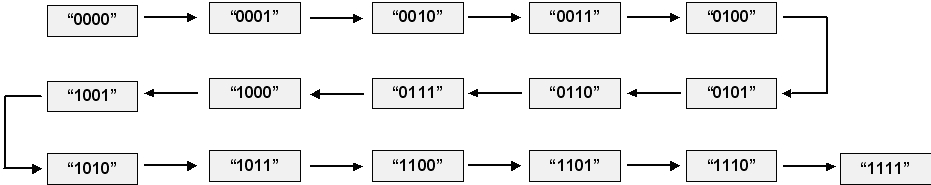
\includegraphics[width=0.80\textwidth]{images/brute_force}
          \caption[Schemat ataku brute-force]{
              źródło: \url{http://m.eet.com/media/1158622/aes_security_fig2.jpg}
            }
            \label{chapter:logs:collecting:brute_force}
        \end{figure}
        
        Jeśli w momencie trwania ataku administrator zdecydowałby się na usunięcie plików z logami, stałoby się niemożliwe wykrycie ataku poprzez analizę logów w poszukiwaniu wzorców właściwych dla rodzaju ataku.
        
        \subsubsection{Rotacja logów}
        \label{chapter:logs:collecting:rotation}
        Rozwiązaniem rosnącego rozmiaru pliku logów jest \textbf{rotacja}. W nowoczesnych systemach logowania
        jest to najczęściej domyślnie zaimplementowanie. \textbf{Rotacja} polega na przekopiowaniu 
        zawartości logów do nowego pliku oraz wyczyszczeniu aktualnego. Kopiowanie jest najczęściej połączone
        z kompresją (\ref{chapter:logs:history:compressed_log_format}), która może zostać wykonana od razu lub po upływie 
        pewnego czasu, kiedy to najstarsze pliki stają się najmniej ważne. Archiwizacja jest tutaj szczególnie istotna, 
        ponieważ skompresowane pliki tekstowe zajmują aż do 90 procent oryginalnego rozmiaru.
        
        Rotacja również nie jest rozwiązaniem idealnym. Staje się ona bezużyteczna jeśli nie jest połączona
        z odpowiednią polityką, polegającą na usuwaniu starych archiwów. Tworzenie kolejnych archiwów,
        szczególnie na maszynie z ograniczoną przestrzenią dyskową, może również doprowadzić do jej wyczerpania.
        Niemniej problem jest tutaj znacznie oddalony w czasie. Istnieje już niebezpieczeństwo przeprowadzania
        ataku na system, gdzie zaimplementowana została rotacja logów. Wymagana on wiedzy na temat działania systemu.
        Odpowiednie stymulowanie systemu mogłoby zaowocować ciągłym zwiększaniem rozmiarów logu, a w dalszej kolejności
        częstszymi rotacjami. Warto w tym miejscu nadmienić, że ta technika archiwizacji jest bardzo często
        połączona z usuwaniem archiwów starszych niż pewien okres czasu lub, co bardziej niebezpieczne, będących
        rezultatem n-tej archiwizacji. Atakujący mógłby zacząć oddziaływać na system w taki sposób, że informacje
        w logach stałyby się powtarzalne i dotyczyłyby tej samej czynności, jaką aplikacja by wykonywała.
        
        \subsubsection{Przesyłanie logów do centralnej lokalizacji}
        \label{chapter:logs:collecting:central_location}
        Centralna agregacja logów jest techniką, którą często stosuje się w połączeniu z rotacją.
        Pierwsza operacja jest istotna z punktu widzenia długofalowego przetwarzania, analizowania oraz
        budowania hurtowni danych, gdzie główną daną, podmiotem jest log. Rotacja natomiast jest skoncentrowana
        na maszynie, na której wygenerowane zostały logi. Jej celem, jak to zostało wspomniane w \ref{chapter:logs:collecting:rotation},
        jest oszczędzanie przestrzeni dyskowej.
    